\begin{figure}[t]
\centering
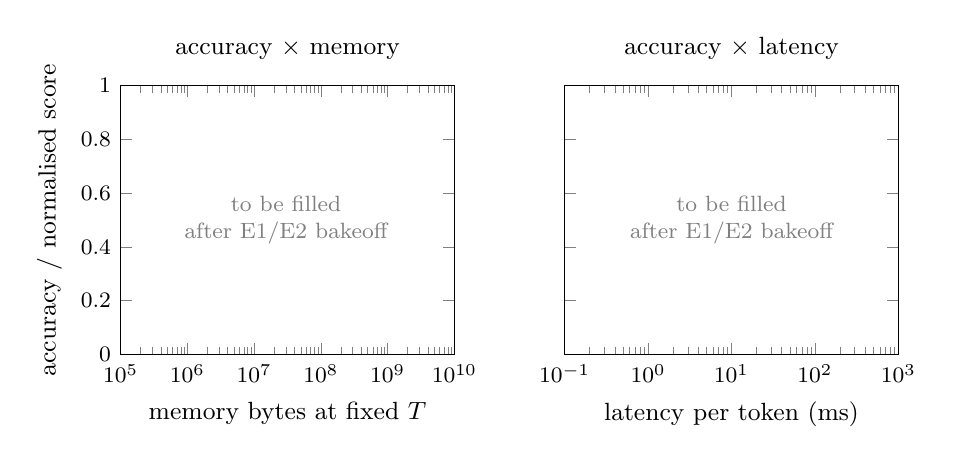
\begin{tikzpicture}
\begin{semilogxaxis}[name=mem,
  width=0.48\linewidth, height=5cm, xmin=1e5, xmax=1e10, ymin=0, ymax=1,
  xlabel={memory bytes at fixed $T$}, ylabel={accuracy / normalised score},
  tick label style={font=\footnotesize}, label style={font=\small}, title={\small accuracy $\times$ memory}]
\node[font=\footnotesize,gray,align=center] at (axis cs:3e7,0.5) {to be filled\\after E1/E2 bakeoff};
\end{semilogxaxis}
\begin{semilogxaxis}[at={(mem.east)},anchor=west,xshift=1.4cm,
  width=0.48\linewidth, height=5cm, xmin=0.1, xmax=1000, ymin=0, ymax=1,
  xlabel={latency per token (ms)}, yticklabels={},
  tick label style={font=\footnotesize}, label style={font=\small}, title={\small accuracy $\times$ latency}]
\node[font=\footnotesize,gray,align=center] at (axis cs:10,0.5) {to be filled\\after E1/E2 bakeoff};
\end{semilogxaxis}
\end{tikzpicture}
\caption{Pareto template (empty by design). Every architecture--scale--seed run of E1/E2 will be one point in both
panels, at the same $T\in\{512,2\text{k},8\text{k},32\text{k}\}$. Non-dominated fronts will be drawn per $T$. Marker
shape will encode architecture and marker size will encode the third axis, so that no single ratio stands in for the front.}
\label{fig:pareto}
\end{figure}
